
% File: template.tex
%
%**************************************************
\documentclass[12pt, a4paper, italian]{scrartcl}

% loading packages
\usepackage[latin1]{inputenc}
\usepackage[english]{babel}
\usepackage{graphics, graphicx}
\usepackage{color}
\usepackage{fancyhdr}
\usepackage{geometry}
\usepackage{rotating, colortbl}
\usepackage{url}

% setting margins
\geometry{left=2cm, right=2cm, top=2.5cm, bottom=3cm}

% caption style
\addtokomafont{caption}{\small}
\setkomafont{captionlabel}{\sffamily\bfseries}

% setting headers and footers
\pagestyle{fancy}
\renewcommand\headrulewidth{.1pt}
\fancyhead[L]{\sffamily University of Trieste}
\fancyhead[C]{\sffamily DIA}
\fancyhead[R]{\sffamily\itshape M. Crosariol}

\renewcommand\footrulewidth{.1pt}
\fancyfoot[l]{\sffamily\itshape Computer Vision and Pattern Recognition}
\fancyfoot[C]{\thepage}
\fancyfoot[R]{\sffamily\itshape Academic year 2024/2025}
%-----------------------------------
% Inizio documento
%-----------------------------------
\begin{document}
%----- Copertina
%**************************************************
% File: copertina.tex
%
% 2005 Mauro Tizianel.
%**************************************************
\begin{titlepage}
{
\title{
	\enlargethispage{0.1\textheight}
	\pagenumbering{arabic}
	\vspace{-1cm}
	%---------- Intestazione
	\begin{center}
		\begin{minipage}{0.20\textwidth}
			\centering
			%\includegraphics[width=0.85\textwidth, bb=0 0 827 827]{fig/logo.png} % Output in DVI
			
\includegraphics[width=0.85\textwidth]{fig/new_logo.png} % Output in PDF
		\end{minipage}
		\begin{minipage}{0.75\textwidth}
			\small
			\begin{flushleft}
				{\sffamily UNIVERSITY OF TRIESTE}
			\end{flushleft}
			\rule{0.95\linewidth}{1.5pt}
			\begin{flushleft}
				{\sffamily DEPARTMENT OF ENGINEERING AND ARCHITECTURE}
			\end{flushleft}		
		\end{minipage}
	\end{center}
	%----------
	\vspace{1cm}
	%----------
	\begin{center}
		{\sffamily\Large Computer Vision and Pattern Recognition}
	\end{center}
	%----------
	\vspace{2.5cm}
	%---------- Titolo
	\begin{center}
	{CVPR 2024 CNN classifier - Project Report}
	\end{center}
	\begin{center}
		\rule{0.95\linewidth}{3pt}
	\end{center}
	\vspace{6cm}
	\begin{center}
		\normalsize
		%----------
		\begin{tabular}{p{0.65\linewidth} p{0.30\linewidth}}
			{\sffamily Professor:}&%
			{\sffamily Student:}\\
			{\sffamily \bfseries Felice Andrea Pellegrino}&%
			{\sffamily \bfseries Matteo Crosariol}\\
			{}&{}\\
		\end{tabular}
	\end{center}
	%----------
	\vspace{1cm}
	%----------
	\begin{center}
		\rule{0.75\linewidth}{1pt}
	\end{center}
	\begin{center}	
		{\normalsize \scshape Academic year 2024/2025}
	\end{center}
}
%----------
\date{}
\author{}
\maketitle
}
\end{titlepage}
%----- Corpo del documento
\newpage
\tableofcontents
\newpage


\section{Problem Statement}
This project requires the implementation of an image classifier based on the
bag-of-words approach. The provided dataset (from [Lazebnik et al., 2006]\cite{Lazebnik:Crosa}),
contains 15 categories (office, kitchen, living room, bedroom, store, industrial,
tall building, inside city, street, highway, coast, open country, mountain, forest,
suburb), and is already divided in training set and test set. Samples are shown
in Fig. 1.

 \begin{figure} [h!]
 \centering
  { 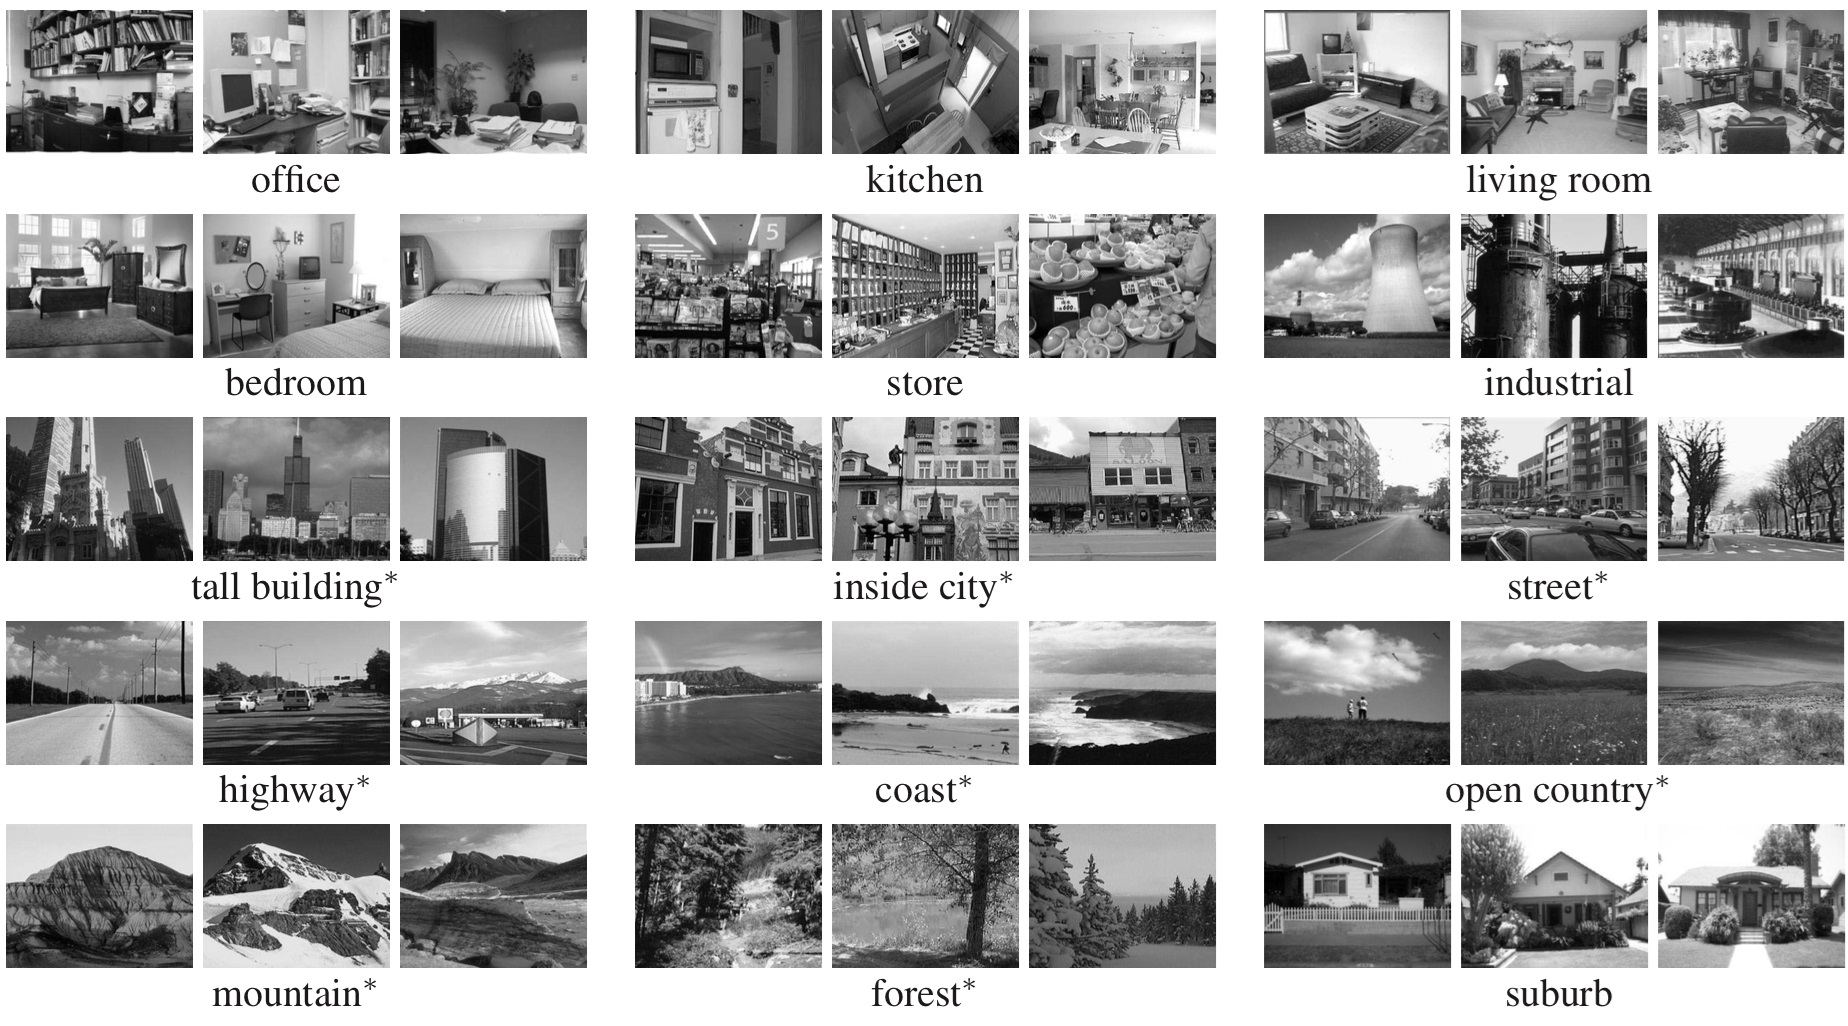
\includegraphics[width=.85\textwidth]{fig/dataset_example.jpg} \caption{Examples of images from each of the 15 categories of the provided dataset (the same as [Lazebnik et al., 2006]).
}} 
  \end{figure}
  


The project mainly is divided in three parts:
\begin{enumerate}
	\item \textbf{Base CNN Classifier}: Initialization and training of a CNN model with a fixed architecture.
	\item \textbf{Improved CNN Classifier}: Optimization of the previous result by making use of data augmentation, regularization and the employment an ensemble of networks (ten), trained independently.
	\item \textbf{Transfer learning based solution}: Improvement on the previous results through transfer learning, by finetuning a pre-trained model to the given dataset.
\end{enumerate}


  \newpage
  \section{Base CNN Classifier}
  \subsection{Task specification}
  The goal of this task is to train a shallow network from scratch according to the following specifications:
\begin{itemize}
	\item the architecture of the network is shown in Table 1;
	\item since the input image is 64x64 it is needed to resize the images in order to feed them to the network;
	\item split the provided training set in 85\% for actual training set and 15\% to be used as validation set;
	\item employ the stochastic gradient descent with momentum optimization algorithm;
	\item use minibatches of size 32;
	\item set the initial bias values to 0 and use initial weights drawn from a Gaussian distribution having a mean of 0 and a standard deviation of 0.01;
\end{itemize}

\begin{table}[h]
\centering
\begin{tabular}{llll}
\hline
 \#&  &Type &Size  \\
 \hline
 1& & Image Input &64x64x1 images  \\
 2&  & Convolution   & 8 3x3 convolutions with stride 1 \\
 3&  & ReLu   & \\
 4&  & Max Pooling   &2x2 max pooling with stride 2 \\
 5&  & Convolution   &16 3x3 convolutions with stride 1 \\
 6&  & ReLu   & \\
 7&  & Max Pooling   &2x2 max pooling with stride 2 \\
 8&  & Convolution   &32 3x3 convolutions with stride 1 \\
 9&  & ReLu   & \\
 10&  & Fully Connected   &15 \\
 11&  & Softmax   &softmax \\
 12&  & Classification Output   &crossentropyex \\
 
\end{tabular}
\caption{Layout of the CNN used in the Base CNN Classifier }
\end{table}

  \subsection{Implementation}
    \subsubsection{Dataset loading and transformations definition}
    \begin{verbatim}
    # Define transformations and datasets
    transform = transforms.Compose([
        transforms.Resize((64, 64)),
        transforms.Grayscale(),
        transforms.ToTensor(), #conversion to tensor.
        transforms.Lambda(lambda x: x * 255)
    ])

\end{verbatim}
This transformation rescales the images anisotropically to a size of 64x64, converts them to grayscale (since they will be loaded as RGB images due to the use of ImageFolder) ,converts them to a tensor and then scales the values back to [0,255] since ToTensor converts the image to a sensor with values in the range [0,1].\newline

After the splitting of the provided training set in 85\% for actual training set and 15\% to be used as validation set and the application of the transformations on the data, the three DataLoaders (train, validation and test) have been created.
   \begin{verbatim}
    full_training_data = datasets.ImageFolder(root="Dataset"+"/train")
    test_dataset = datasets.ImageFolder(root="Dataset"+"/test")
    full_training_data.transform=transform
    test_dataset.transform=transform

    train_size = int(SPLIT_RATIO_TRAINING * len(full_training_data))
    val_size = len(full_training_data) - train_size
    train_dataset, val_dataset = torch.utils.data.random_split(full_training_data, 
    [train_size, val_size])
    train_loader = DataLoader(train_dataset, batch_size=BATCH_SIZE, shuffle=True)
    validation_loader = DataLoader(val_dataset, batch_size=BATCH_SIZE, shuffle=True)
    test_loader = DataLoader(test_dataset, batch_size=BATCH_SIZE, shuffle=True)
\end{verbatim}
 \subsubsection{Model implementation and initialization}
 The architecture of the network is implemented using PyTorch:
    \begin{verbatim}
	self.layers = nn.Sequential(
	  	nn.Conv2d(in_channels=1, out_channels=8,kernel_size=3,stride=1, padding=1),
	  	nn.ReLU(),
	  	nn.MaxPool2d(kernel_size=2, stride=2),
	  	nn.Conv2d(in_channels=8, out_channels=16, kernel_size=3,stride=1, padding=1),
	  	nn.ReLU(),
	  	nn.MaxPool2d(kernel_size=2, stride=2),
	  	nn.Conv2d(in_channels=16, out_channels=32, kernel_size=3,stride=1, padding=1),
	  	nn.ReLU(),
	  	nn.Flatten(),
	  	nn.Linear(in_features=self.last_input_size, out_features=15)
	)
\end{verbatim}
While the Convolutional and Linear layers are then initialized with the following code:
    \begin{verbatim}
        if type(model) == nn.Conv2d or type(model) == nn.Linear:
            nn.init.normal_(model.weight, mean=0.0, std=0.01)
            if model.bias is not None:
                nn.init.constant_(model.bias, 0.0)
\end{verbatim}
  \newpage
  \subsubsection{Training and Validation}
  Regarding the training the parameters used are:
  \begin{itemize}
	\item \textbf{Learning rate}:0.001. This value has been chosen after some trial, it's not too big to overshoot nor too small to slow down the training too much;
	\item \textbf{Momentum}: 0.9. This value helps the model converge faster and avoid getting stuck in local minima. 
\end{itemize}
In addition, in order to stop the training before reaching the epochs limit the parameter \textbf{no\_improvement\_counter} is used. Its value is 15 and it describes the number of epochs without improvement after which the training is stopped using the validation loss as a stopping criterion.

  Firs of all the model has to be initialized,after that the optimizer (stochastic gradient descent) and the loss function (cross entropy) are defined:
\begin{verbatim} 
      model = CNN_task_1()
      optimizer = torch.optim.SGD(model.parameters(), lr=0.001,momentum=0.9) 
      loss = torch.nn.CrossEntropyLoss()
\end{verbatim}

For each epoch the model is trained, and the training and validation losses and accuracies are calculated in order track the best performance (based on validation), and save the model.

\begin{verbatim} 
 		#TRAINING
        model.train(True)
        for x, y in iter(train_loader):
            optimizer.zero_grad()
            y_pred = model(x)
            l = loss(y_pred, y) #compute the loss
            l.backward() #backward pass
            optimizer.step() #update the weights

        training_loss, training_accuracy = calculate_loss_accuracy(model, train_loader,
         loss)
\end{verbatim}
\begin{verbatim} 
        #VALIDATION
        model.eval()
        with torch.no_grad():
            validation_loss, validation_accuracy = calculate_loss_accuracy(model,
             validation_loader, loss)
            validation_losses.append(validation_loss)
            validation_accuracies.append(validation_accuracy)
            if validation_loss < best_validation_loss:
                print(f"!!! NEW BEST MODEL FOUND")
                best_model = model.state_dict()
                best_validation_loss = validation_loss
                no_improvement_counter=0
            else:
                no_improvement_counter +=1
                if no_improvement_counter==15: #stop validation 
                    break #exit here
\end{verbatim}
    \newpage
  \subsubsection{Testing}
  Load the best model and evaluate the performance on the test set:
  
  \begin{verbatim} 
    #LOAD THE BEST MODEL
    model.load_state_dict(best_model)
    torch.save(best_model, "models_1.pt")
    
    #TEST MODEL
    total = 0
    correct = 0
    all_predictions = []
    all_labels = []
    with torch.no_grad():
        for x_test, y_test in test_loader:
            y_pred_test = model(x_test)
            _, predicted = torch.max(y_pred_test.data, 1)
            total += y_test.size(0)
            correct += (predicted == y_test).sum().item()
            all_predictions.extend(predicted.numpy())
            all_labels.extend(y_test.numpy())

    test_accuracy = 100 * correct / total
\end{verbatim}

 \subsection{Results}
 \begin{figure} [h!]
 \centering
  { 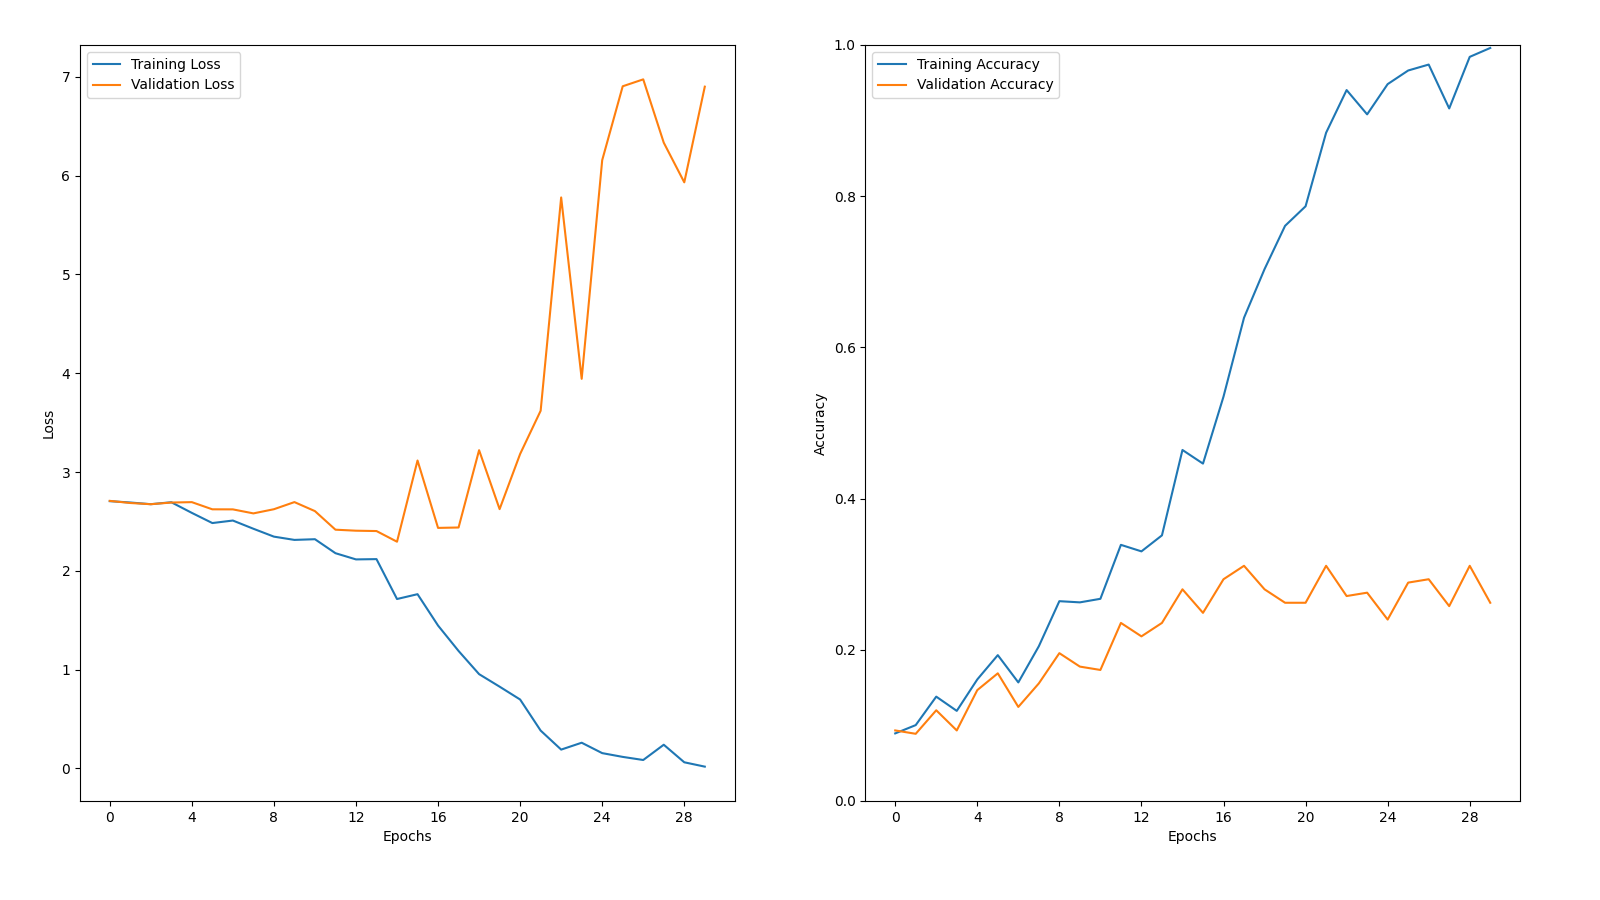
\includegraphics[width=.85\textwidth]{fig/loss_and_accuracy_task_1.png} \caption{Training and validation losses and accuracies of the base CNN classifier.
}} 
  \end{figure}
  It can be seen that after few epochs while the training accuracy decrease, the validation accuracy start increasing,so the model quickly starts overfitting.
 \newpage
 
  \begin{figure} [h!]
 \centering
  { 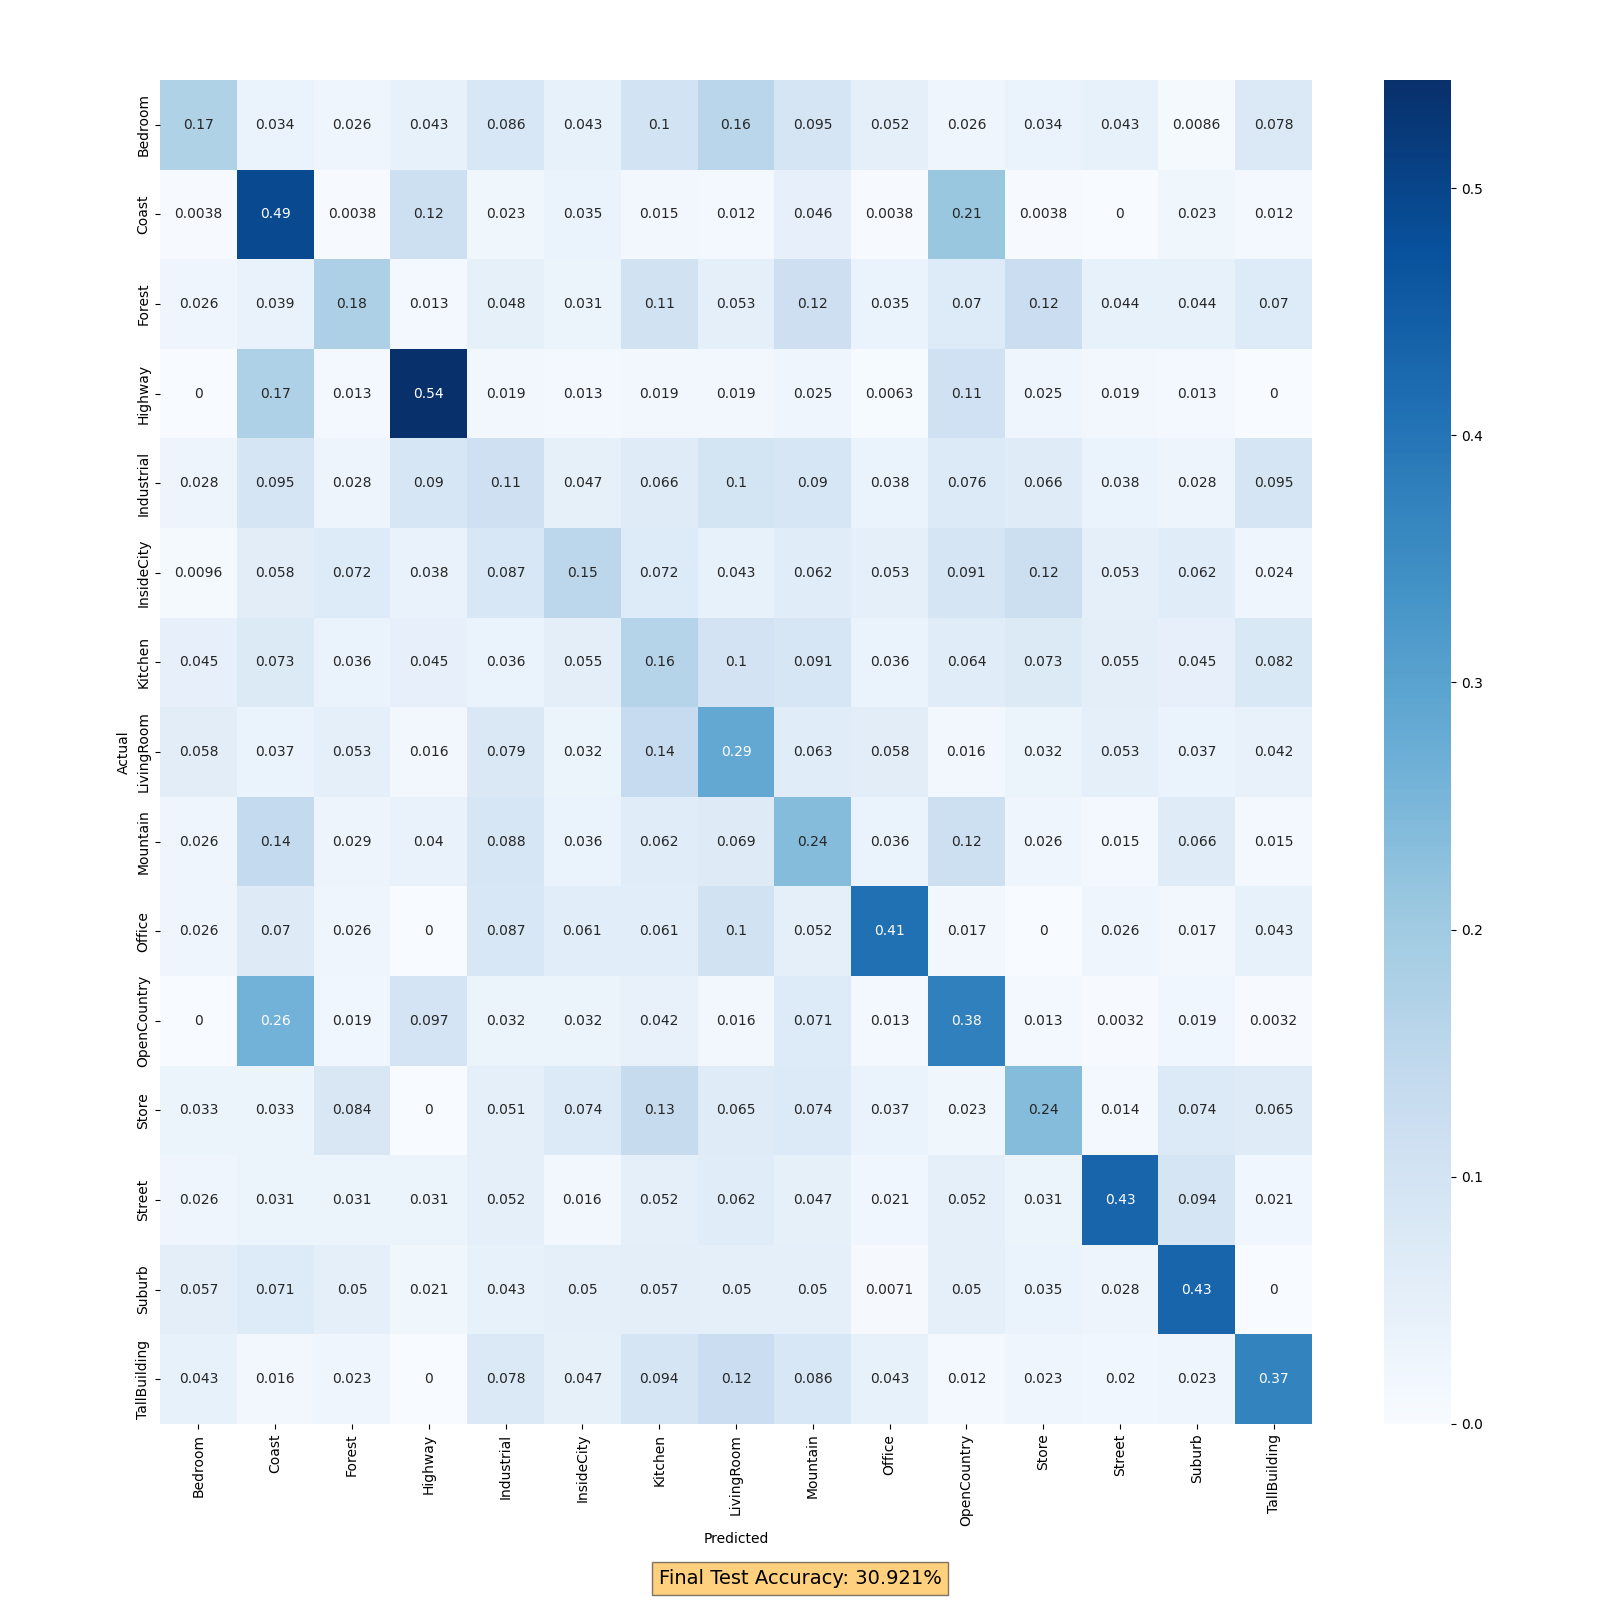
\includegraphics[width=.85\textwidth]{fig/confusion_matrix_task_1.png} \caption{Confusion matrix of the base CNN classifier on the test set.
}} 
  \end{figure}
  
The test accuracy of the model is about 30\%.
From the confusion matrix, it's clear that the model is more precise in categorizing images that belong to certain classes, in fact it seems like the model is more precise in categorizing images referred to open spaces respect to the others. 
  
  
    \newpage
    \section{Improved CNN Classifier}
The goal of this task is to improve the previous result, according to different techniques and modifications, in fact this task has been divided in three different subtasks:
\begin{enumerate}
	\item \textbf{Data augmentation}: applied to the training set in order to improve
the generalization of the model.
	\item \textbf{Regularization and Architectural changes: }: applied to the model in order to improve the performance and to prevent overfitting.
	\item \textbf{Ensemble of networks}: Use an ensemble of networks (ten), trained independently in order to improve the performance.
\end{enumerate}

     
     \subsection{Data augmentation}
      \subsubsection{Task specification}
The following data augmentation techniques have been applied to the training set:   
    \begin{itemize}
	\item Random crop: The image is randomly cropped first into a 180x180 image;
	\item Rescaling: The image is resized to 64x64;
	\item Random horizontal flip: The image is flipped horizontally with a probability of 0.5.
	\item Random rotation: The image is rotated by a random angle between -15 and 15 degrees;
\end{itemize} 
For which regarding the learning rate parameter and the momentum parameter are 0.001 and 0.9 respectively.
In order to stop the training before reaching the epochs limit the parameter \textbf{no\_improvement\_counter} is used and Its value is 25.

  \subsubsection{Implementation}
  According to the techniques described above the transformation applied to the training set are:
   \begin{verbatim} 
       data_augmentation_transform = transforms.Compose([
        transforms.RandomCrop(180),              
        transforms.Resize((64, 64)),
        transforms.RandomHorizontalFlip(p=0.5),       
        transforms.RandomRotation(degrees=15),  
        transforms.Grayscale(),
        transforms.ToTensor(),  
    ])
   \end{verbatim}
   
   \newpage
    \subsubsection{Result}
             \begin{figure} [h!]
 \centering
  { 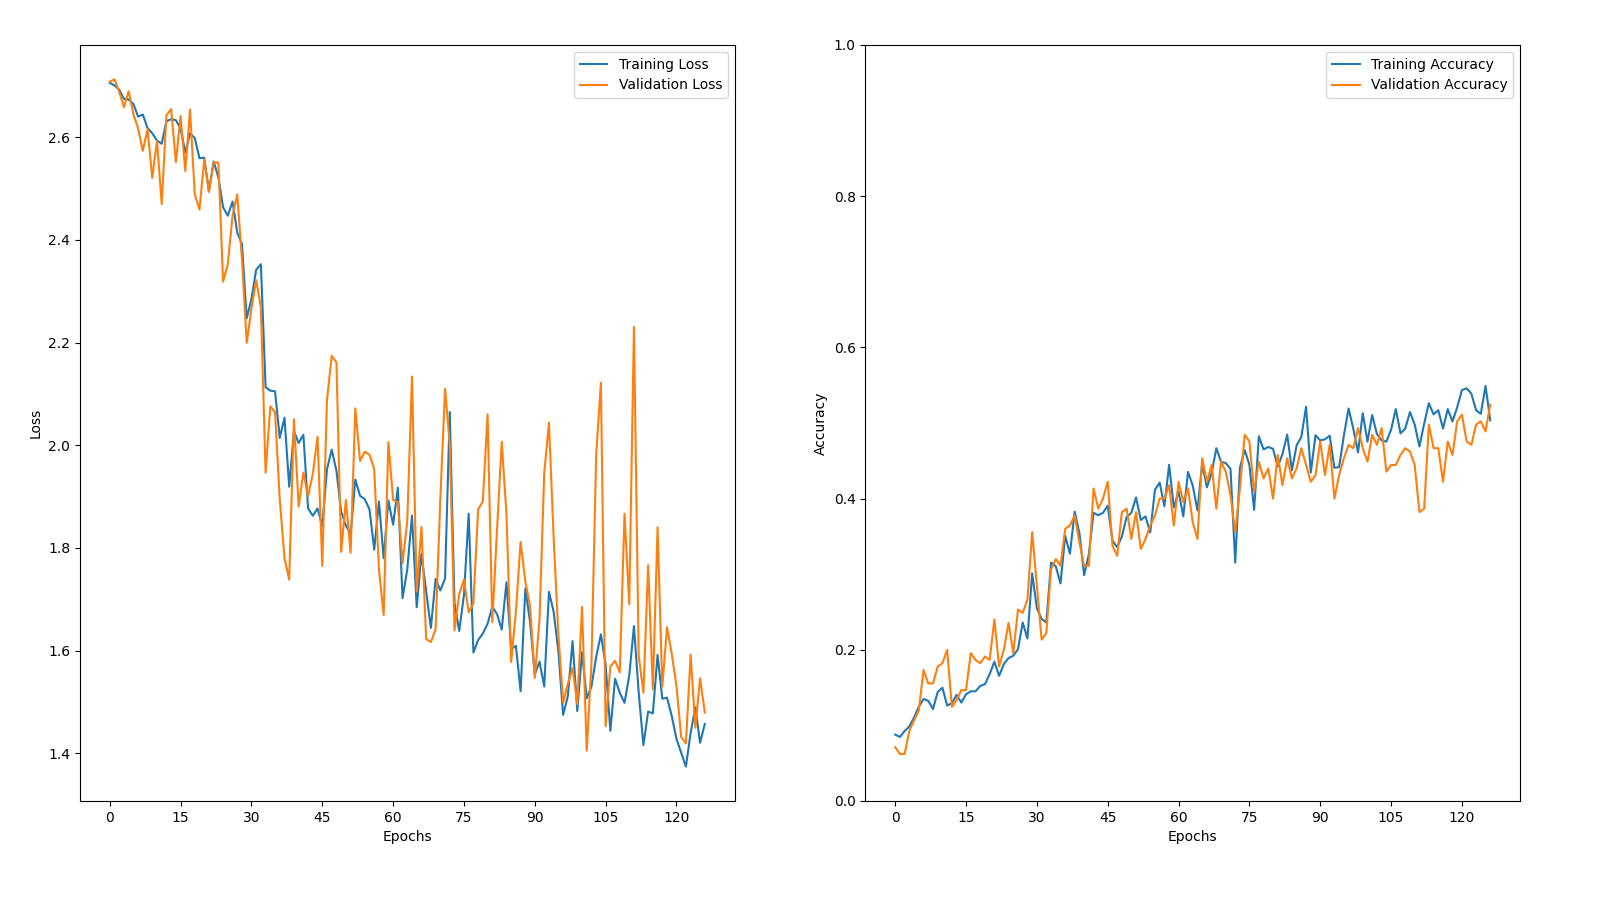
\includegraphics[width=.65\textwidth]{fig/loss_and_accuracy_task_2_individual_network_aug.png} \caption{Training and validation losses and accuracies of the improved CNN classifier with only data augmentation.
}} 
  \end{figure}
  \begin{figure} [h!!!]
 \centering
  { 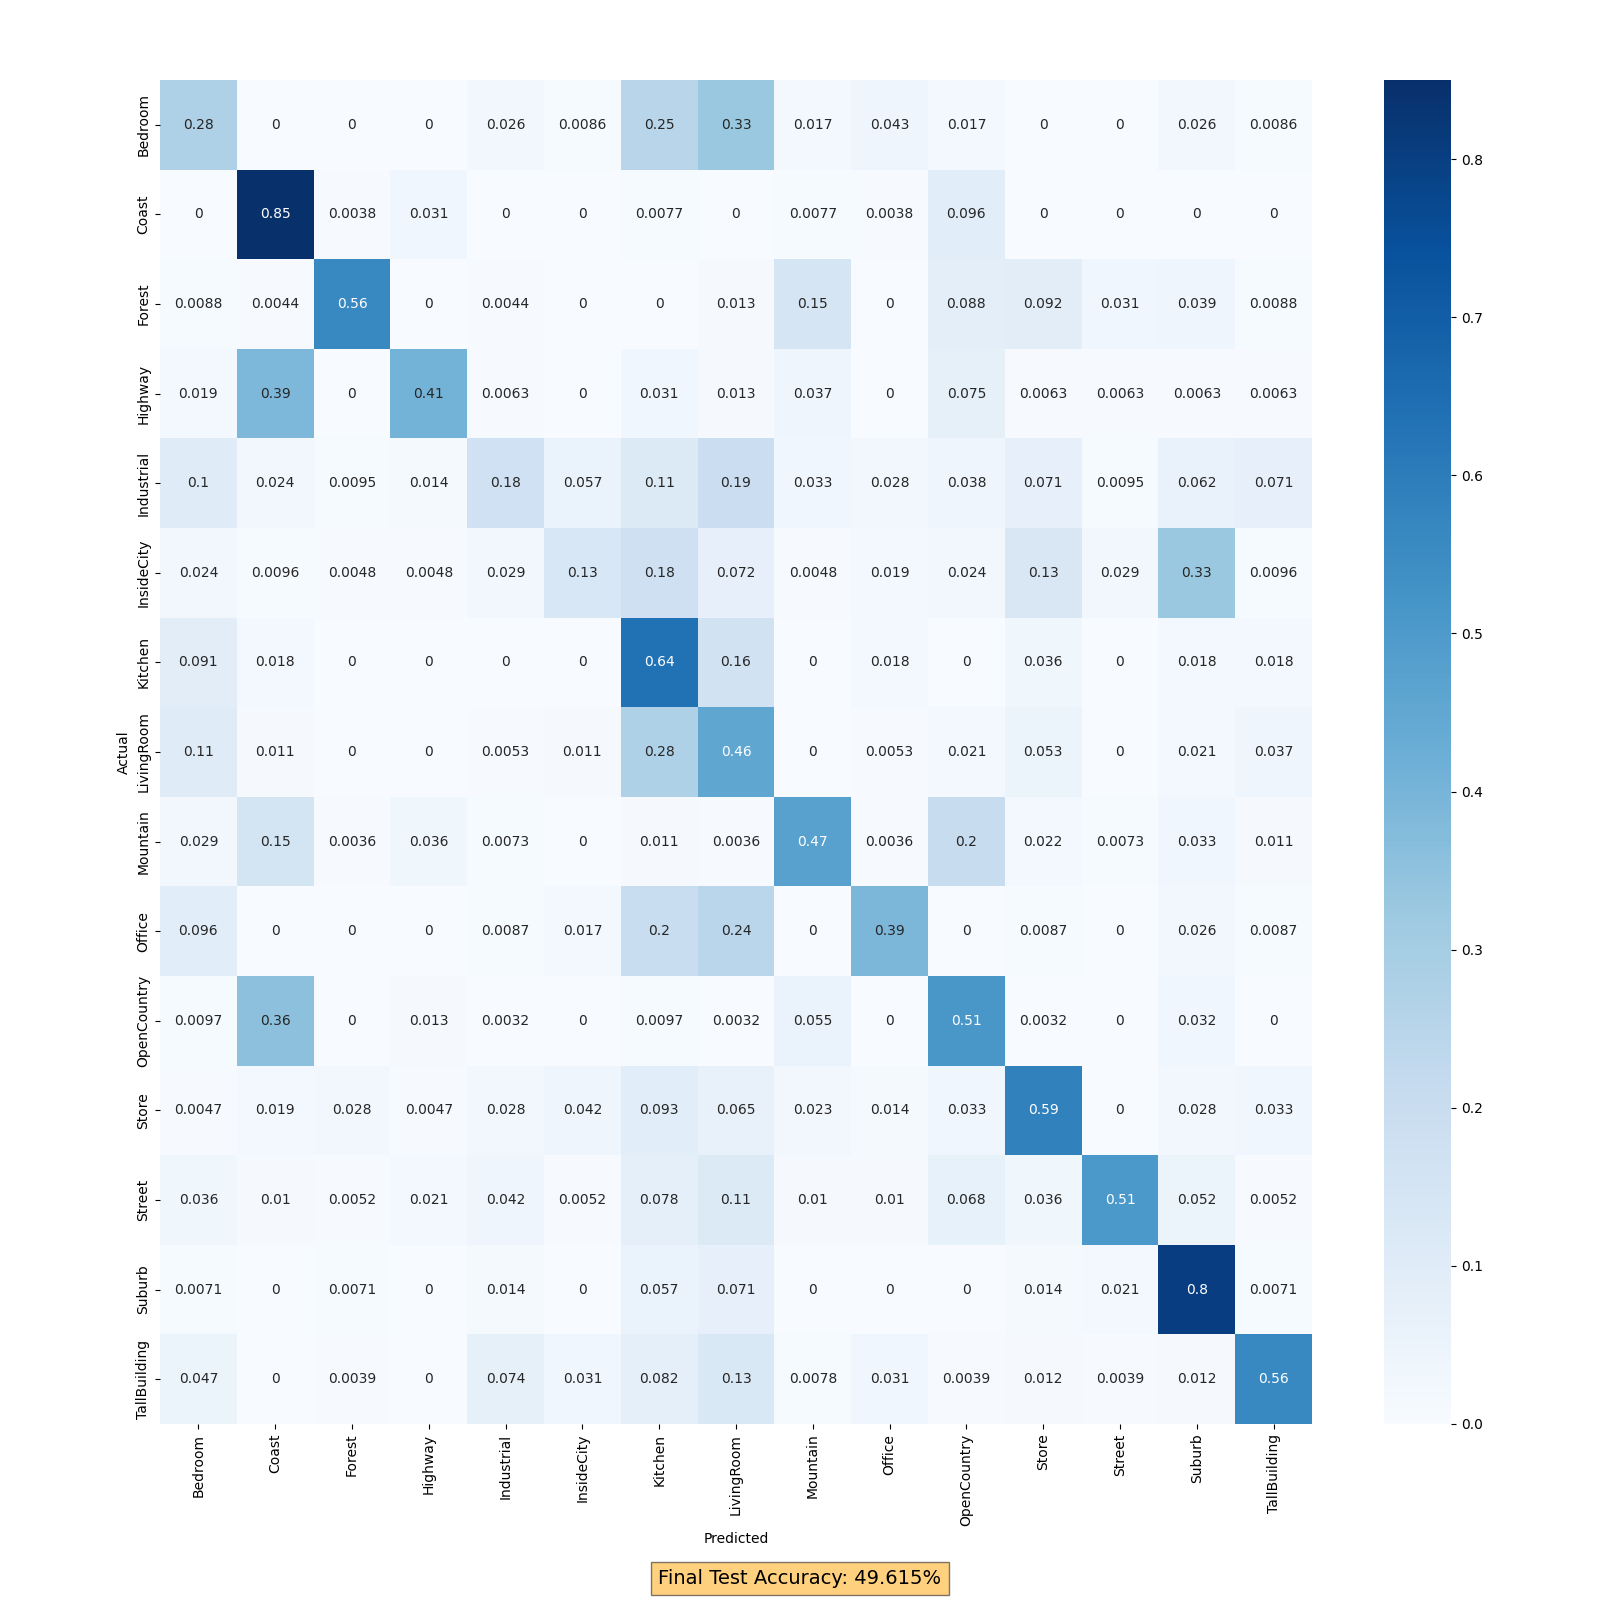
\includegraphics[width=.70\textwidth]{fig/confusion_matrix_task_2_individual_network_aug.png} \caption{Confusion matrix of the improved CNN classifier with only data augmentation.
}} 
  \end{figure}  
The test accuracy of the model is about 49\% which is good improvement from the previous case and also now there is no more overfitting.
Implementing some data augmentation that lead to improve generalization is a good point of start for improving the model.

\newpage
    
    \subsection{Regularization and Architectural changes}
    \subsubsection{Task specification}
    In adding to the data augmentation presented before in this subtask there are the following arrangements:
    \begin{itemize}
	\item batch normalization [Ioffe and Szegedy, 2015]\cite{Ioffe:Szegedy} : add batch normalization layers before the reLU layers;
	\item dropout: add some dropout layer to improve regularization, the dropout rate has been set to 0.1;
	\item Data normalization: The image is normalized with mean 0.5 and standard deviation 0.5;
\end{itemize} 

For which regarding the learning rate parameter and the momentum parameter are 0.001 and 0.9 respectively.
In order to stop the training before reaching the epochs limit the parameter \textbf{no\_improvement\_counter} is used and Its value is 25.


\subsubsection{Implementation}
The architecture of this new improved network is:
\begin{verbatim} 
self.layers = nn.Sequential(
   	nn.Conv2d(in_channels=1, out_channels=8, kernel_size=3, stride=1, padding=1),
   	nn.BatchNorm2d(8),
   	nn.ReLU(),
   	nn.Dropout(.1),
   	nn.MaxPool2d(kernel_size=2, stride=2),
   	nn.Conv2d(in_channels=8, out_channels=16, kernel_size=3, stride=1, padding=1),
   	nn.BatchNorm2d(16),
   	nn.ReLU(),
   	nn.Dropout(.1),
   	nn.MaxPool2d(kernel_size=2, stride=2),
   	nn.Conv2d(in_channels=16, out_channels=32, kernel_size=3, stride=1, padding=1),
   	nn.BatchNorm2d(32),
   	nn.ReLU(),
   	nn.Flatten(),
   	nn.Linear(in_features=self.last_input_size, out_features=15)
)
\end{verbatim}

    \subsubsection{Result}
    The test accuracy of the model is about 57\% which is good improvement from the previous case and there is no overfitting.
From the confusion matrix, it's clear that the model is more precise but it seems that the model has still some difficult to classify the images that belongs to similar category, for examble the interior spaces like bedroom, office, kitchen,store and living room.
\newpage
         \begin{figure} [h!]
 \centering
  { 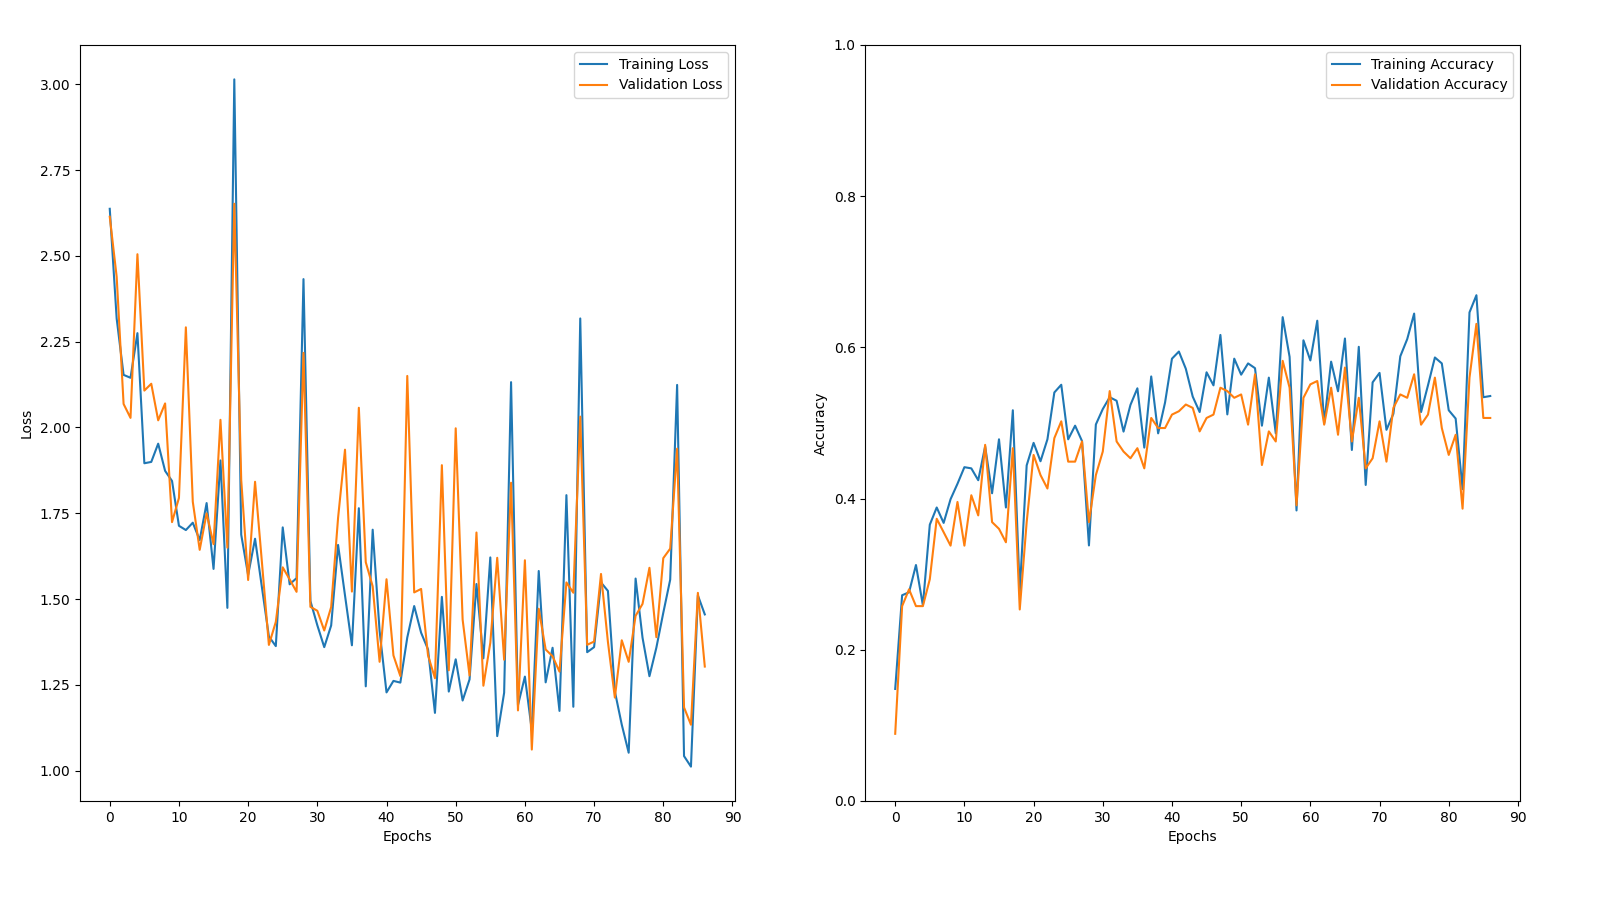
\includegraphics[width=.75\textwidth]{fig/loss_and_accuracy_task_2_individual_network.png} \caption{Training and validation losses and accuracies of the improved CNN classifier.
}} 
  \end{figure}
 
  \begin{figure} [h!]
 \centering
  { 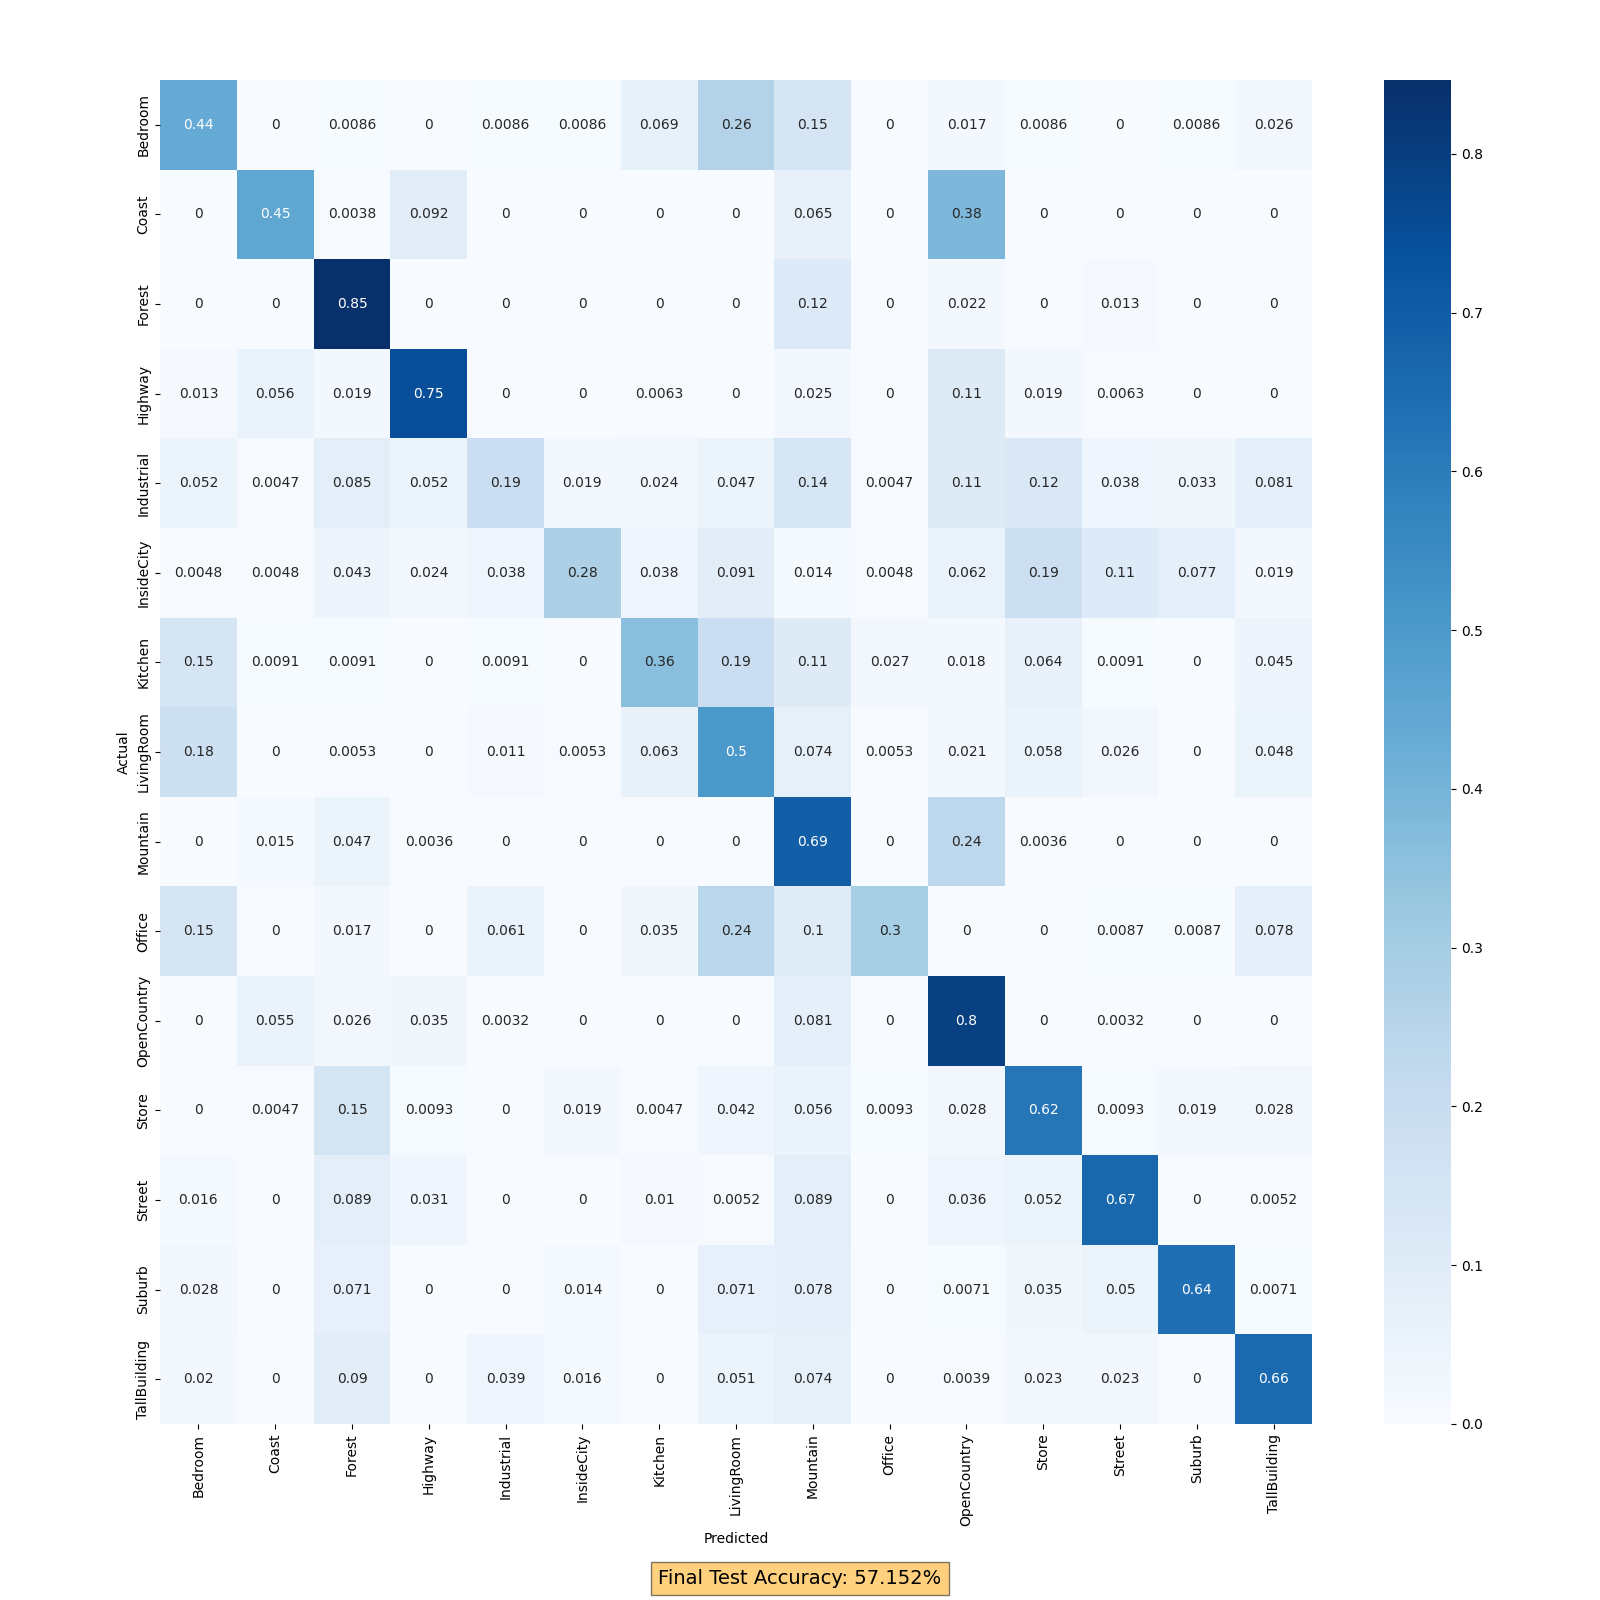
\includegraphics[width=.75\textwidth]{fig/confusion_matrix_task_2_individual_network.png} \caption{Confusion matrix of the improved CNN classifier.
}} 
  \end{figure}
  


\newpage

    \subsection{Ensemble of networks}
    \subsubsection{Task specification}
The goal of this subtask is to employ an ensemble of networks (ten), trained independently and to use the arithmetic average of the outputs to assign the class, as in [Szegedy et al., 2015].\cite{Szegedy:Szegedy}. The network architecture used is the same as the one of the previous subtask.

For which regarding the learning rate parameter and the momentum parameter are 0.001 and 0.9 respectively.
In order to stop the training before reaching the epochs limit the parameter \textbf{no\_improvement\_counter} is used and Its value is 50.

\subsubsection{Implementation}
The architecture of this new improved network is:
\begin{verbatim} 
class ensemble(nn.Module):
    def __init__(self, number_of_networks : int):
        super().__init__()

        self.models = nn.ModuleList([
            CNN_task_2() for _ in range(number_of_networks)])

    def forward(self, x):
        outputs = [model(x) for model in self.models]
        return sum(outputs) / len(outputs)
        )
\end{verbatim}

And after that there is the training of the networks independently:
\begin{verbatim} 
    model =ensemble(number_of_networks)
    no_improvement_counter_limit= int (50)

    loss = torch.nn.CrossEntropyLoss()
    optimizer = [torch.optim.SGD(model_voter.parameters(), lr=0.002, momentum=0.9)
     for model_voter in model.models]


    for epoch in range(EPOCHS_LIMIT):
        #TRAINING
        print('EPOCH {}:'.format(epoch+ 1))

        for i, model_voter in enumerate(model.models):
            #train one epoch
            model_voter.train(True)
            for x, y in iter(train_loader):
                optimizer[i].zero_grad()
                y_pred = model_voter(x)
                l = loss(y_pred, y) #compute the loss
                l.backward() #backward pass
                optimizer[i].step() #update the weights

\end{verbatim}

    \subsubsection{Result}
    The test accuracy of the model is about 61\%, a result that is slight better from the previous case test and still there is not overfitting.
It follows from the matrix that the previous problem of categorization of the images belonging to interior space is still present.
     \begin{figure} [h!]
 \centering
  { 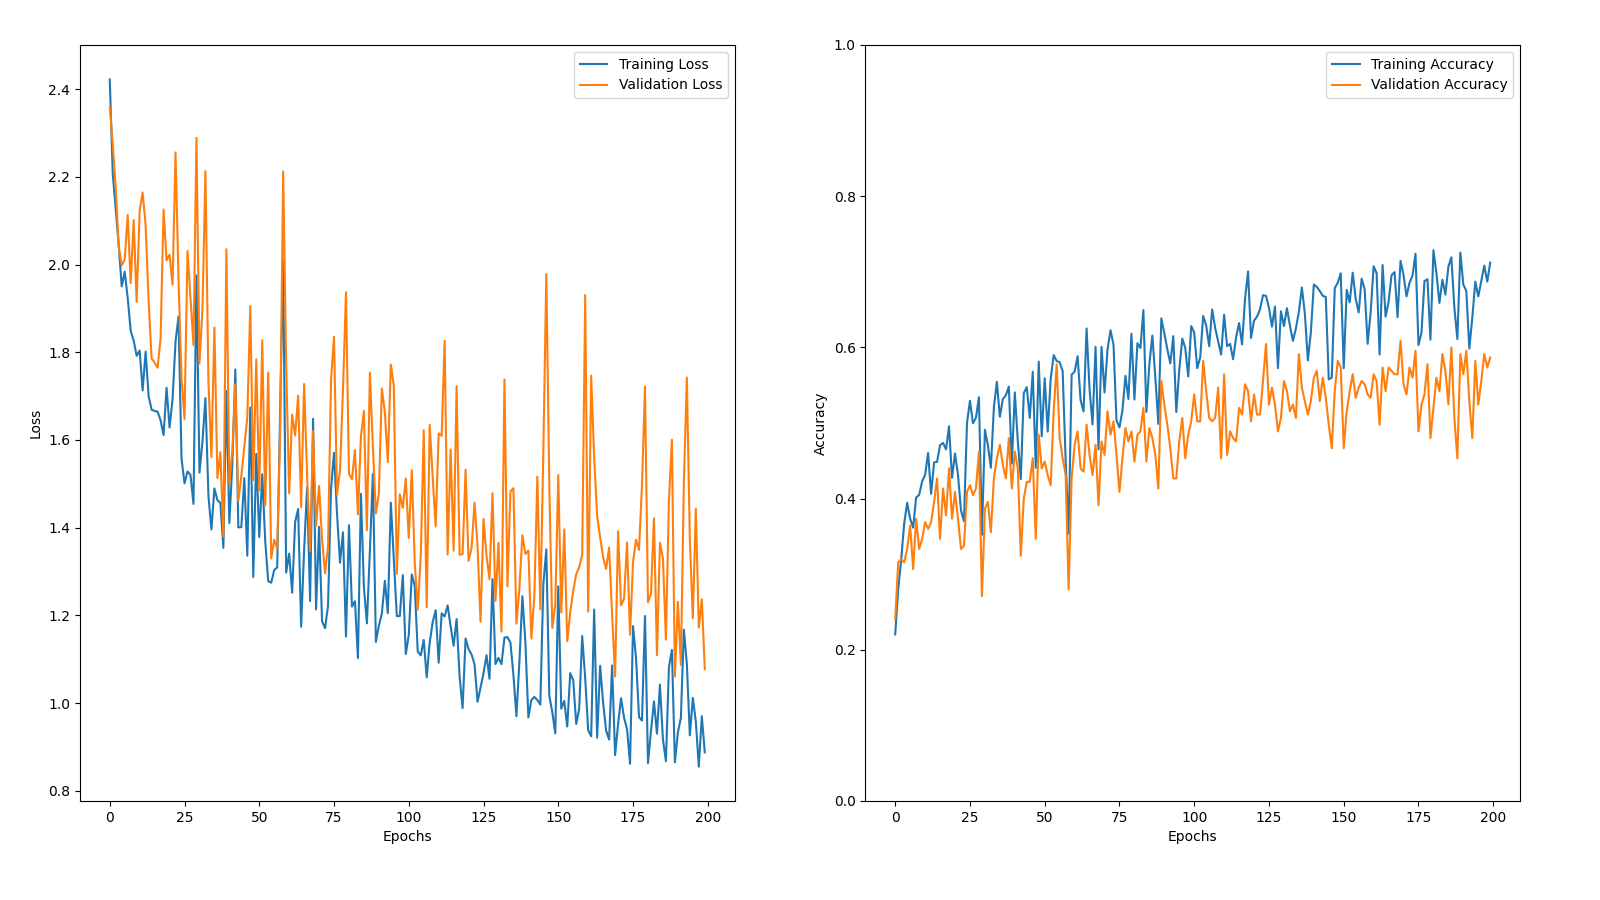
\includegraphics[width=.70\textwidth]{fig/loss_and_accuracy_task_2_ensemble_of_networks.png} \caption{Training and validation losses and accuracies of the results of ten ensemble networks trained independently.
}} 
  \end{figure}
 
  \begin{figure} [h!!!]
 \centering
  { 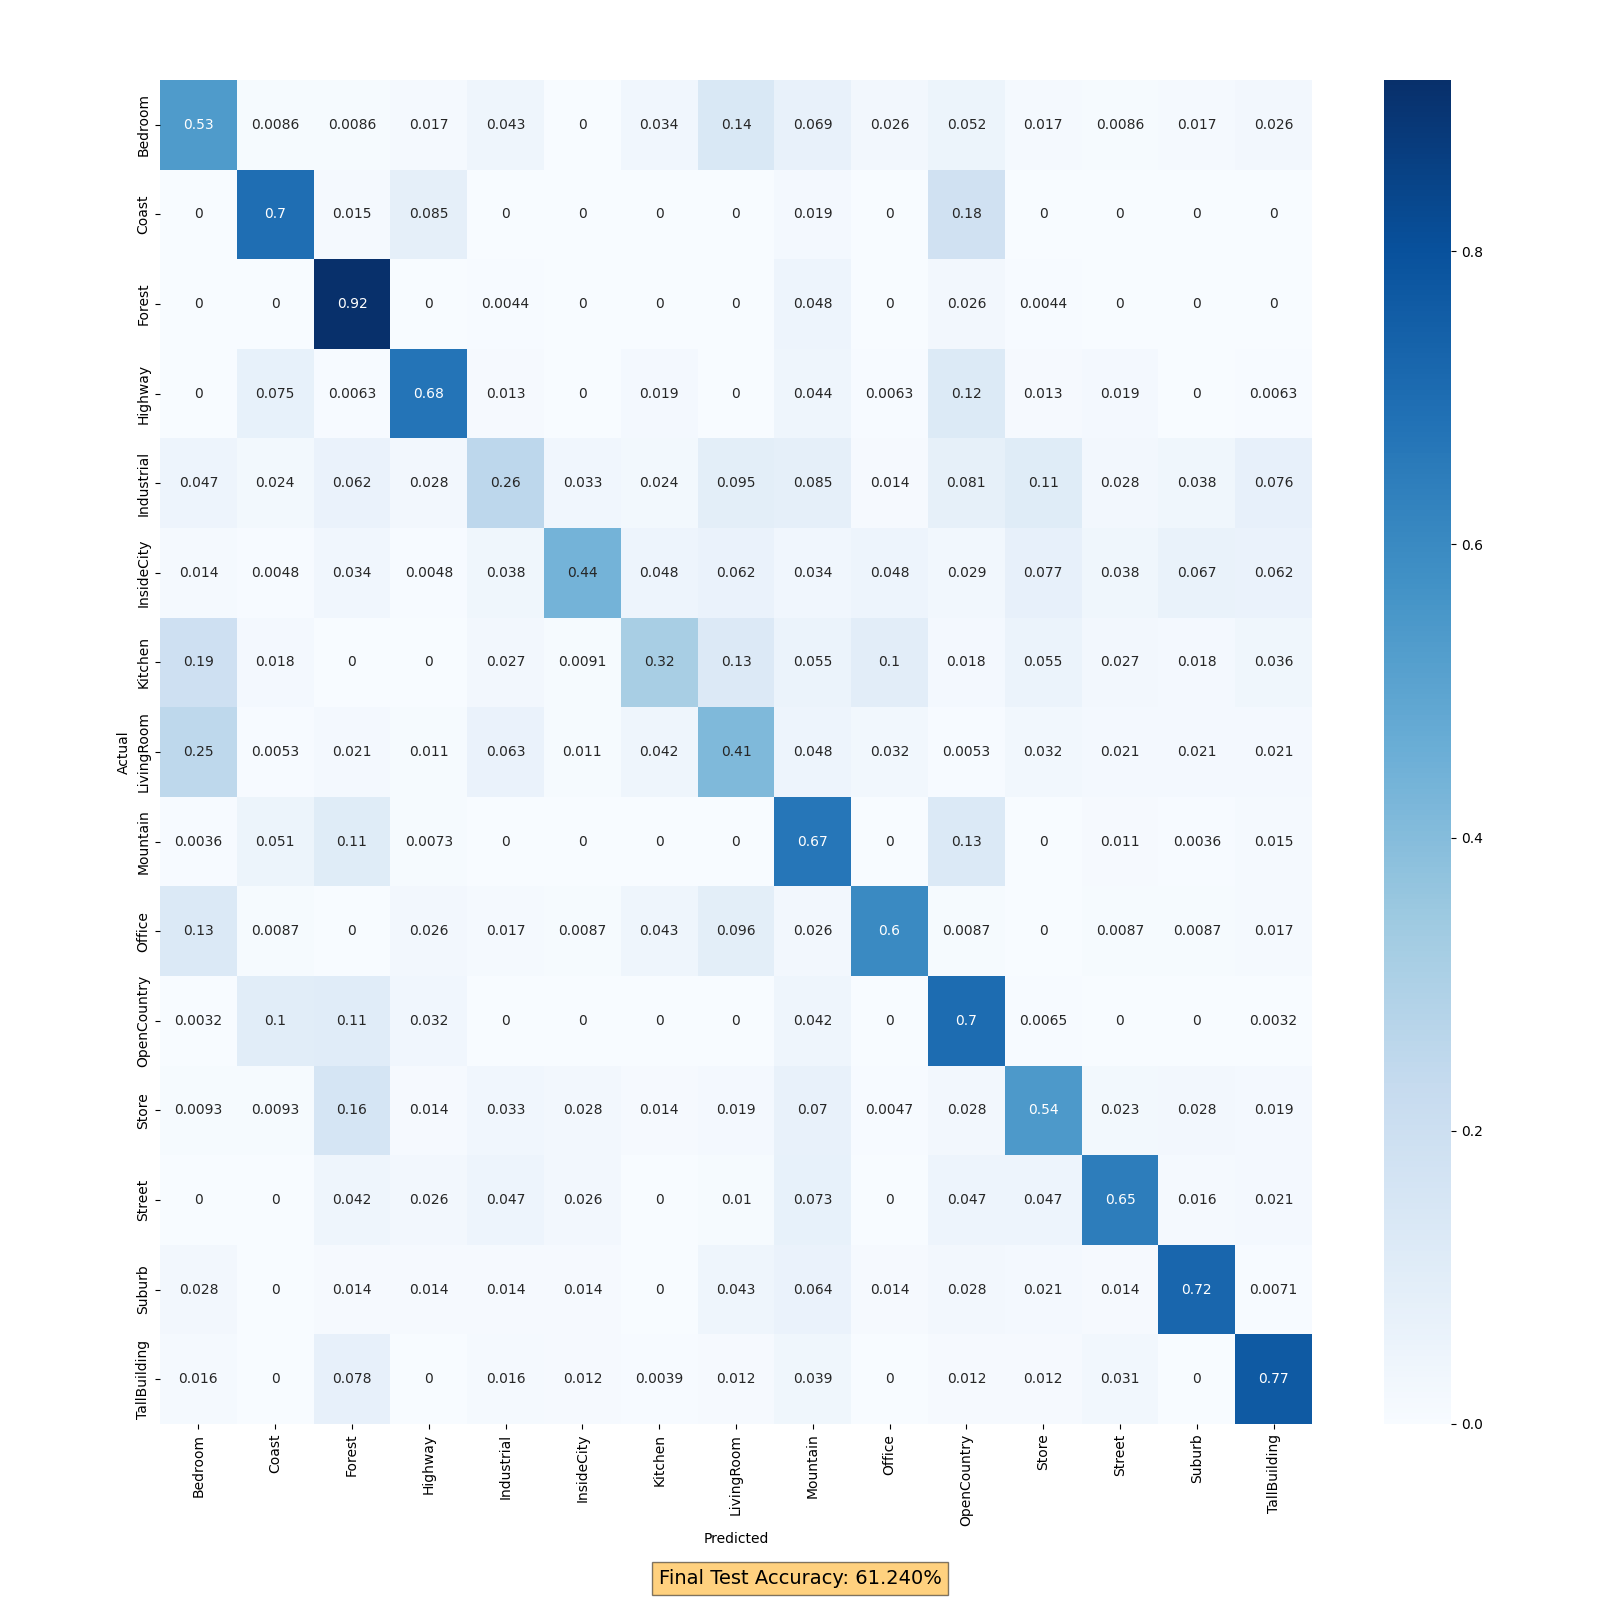
\includegraphics[width=.65\textwidth]{fig/confusion_matrix_task_2_ensemble_of_networks.png} \caption{Confusion matrix of the results of ten ensemble networks trained independently on the test set.
}} 
  \end{figure}
  
  \newpage
  

    
    \newpage
    \section{Transfer learning based solution}
Use transfer learning based on a pre-trained network,AlexNet [Krizhevsky et al., 2012] \cite{Krizhevsky:Krizhevsky}, in the following manner:
\begin{itemize}
	\item freeze the weights of all the layers but the last fully connected layer
and fine-tune the weights of the last layer based on the same train
and validation sets employed before;
\end{itemize} 

    \subsection{Task specification}
According to the use of the AlexNet model our dataset need some transformation.
The images need to be resized to 224x224, duplicated 3 times because of the architecture and characteristics of the model, and the images need to normalized  with the mean and standard deviation of the dataset used for training the model.

For which regarding the learning rate parameter and the momentum parameter are 0.001 and 0.9 respectively.
In order to stop the training before reaching the epochs limit the parameter \textbf{no\_improvement\_counter} is used. Its value is 25 and it describes the number of epochs without improvement after which the training is stopped using the validation loss as a stopping criterion.

\subsection{Task specification}
The data transform for the validation and test dataset is defined ad follows:
    \begin{verbatim} 
    transform = transforms.Compose([
        transforms.Resize((224, 224)),
        transforms.Grayscale(num_output_channels=3),
        transforms.ToTensor(),
        transforms.Normalize(mean=[0.485, 0.456, 0.406], std=[0.229, 0.224, 0.225])             # Normalize image to ImageNet mean and std
    ])
\end{verbatim}

while the data transform for the training set is defined as follows:
    \begin{verbatim} 
    data_augmentation_transform = transforms.Compose([
        transforms.RandomHorizontalFlip(p=0.5),                                                      
        transforms.RandomRotation(degrees=15),                                                  
        transforms.RandomChoice([                                                                
            transforms.Resize((224, 224)),
            transforms.Resize((224, 224)),
            transforms.Compose([
                transforms.RandomCrop(180),
                transforms.Resize(224)
            ])
        ]),
        transforms.Grayscale(num_output_channels=3),
        transforms.ToTensor(),
        transforms.Normalize(mean=[0.485, 0.456, 0.406], std=[0.229, 0.224, 0.225])             # Normalize image to ImageNet mean and std
    ])
\end{verbatim}
  \newpage    
  
For which regarding the model, its weights have to be frozen, except for the classifier?s. Its implementation is :
    \begin{verbatim} 
    def __init__(self, mean_initialization : float = 0.0, 
    std_initialization : float = 0.01):
        super().__init__()

        self.mean_initialization = mean_initialization
        self.std_initialization = std_initialization

        self.alexnet = models.alexnet(weights=AlexNet_Weights.DEFAULT)
        self.alexnet.classifier[6] = nn.Linear(4096, 15)
        # Freeze all layers except the last one:
        for param in self.alexnet.parameters():
            param.requires_grad = False
        self.alexnet.classifier[6].apply(self._init_weights)
        self.alexnet.classifier[6].requires_grad = True
        self.alexnet.classifier[6].weight.requires_grad = True
        self.alexnet.classifier[6].bias.requires_grad = True
\end{verbatim}

\subsection{Result}
 \begin{figure} [h!]
 \centering
  { 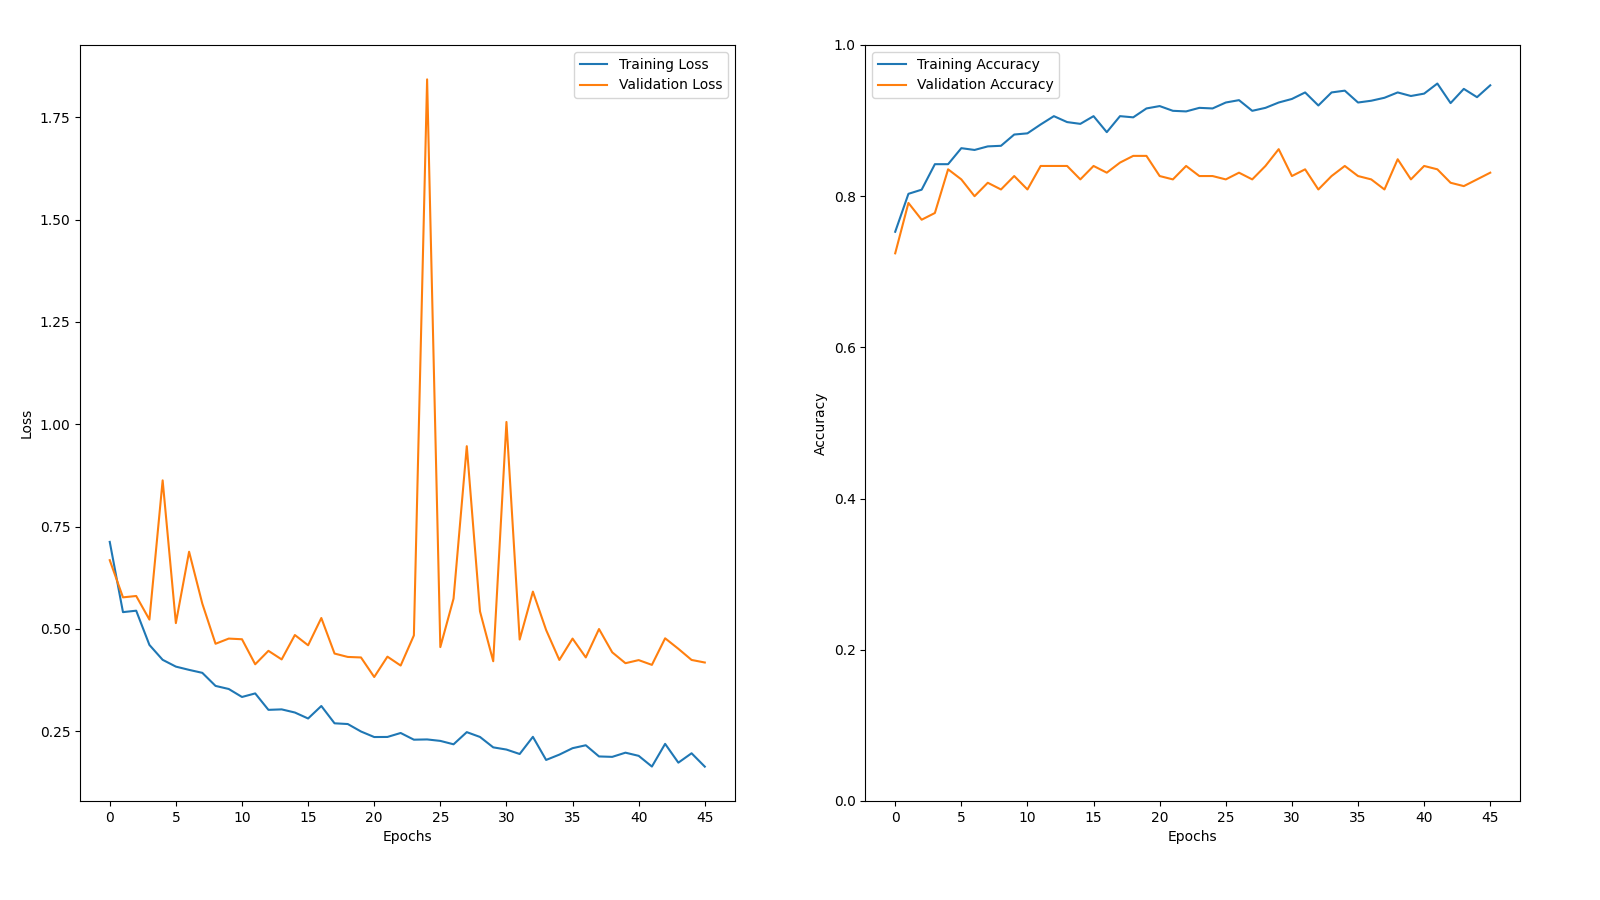
\includegraphics[width=.85\textwidth]{fig/loss_and_accuracy_task_3.png} \caption{Training and validation losses and accuracies of the CNN classifier with AlexNet as a pretrained network.
}} 
  \end{figure}

 \newpage
 
  \begin{figure} [h!]
 \centering
  { 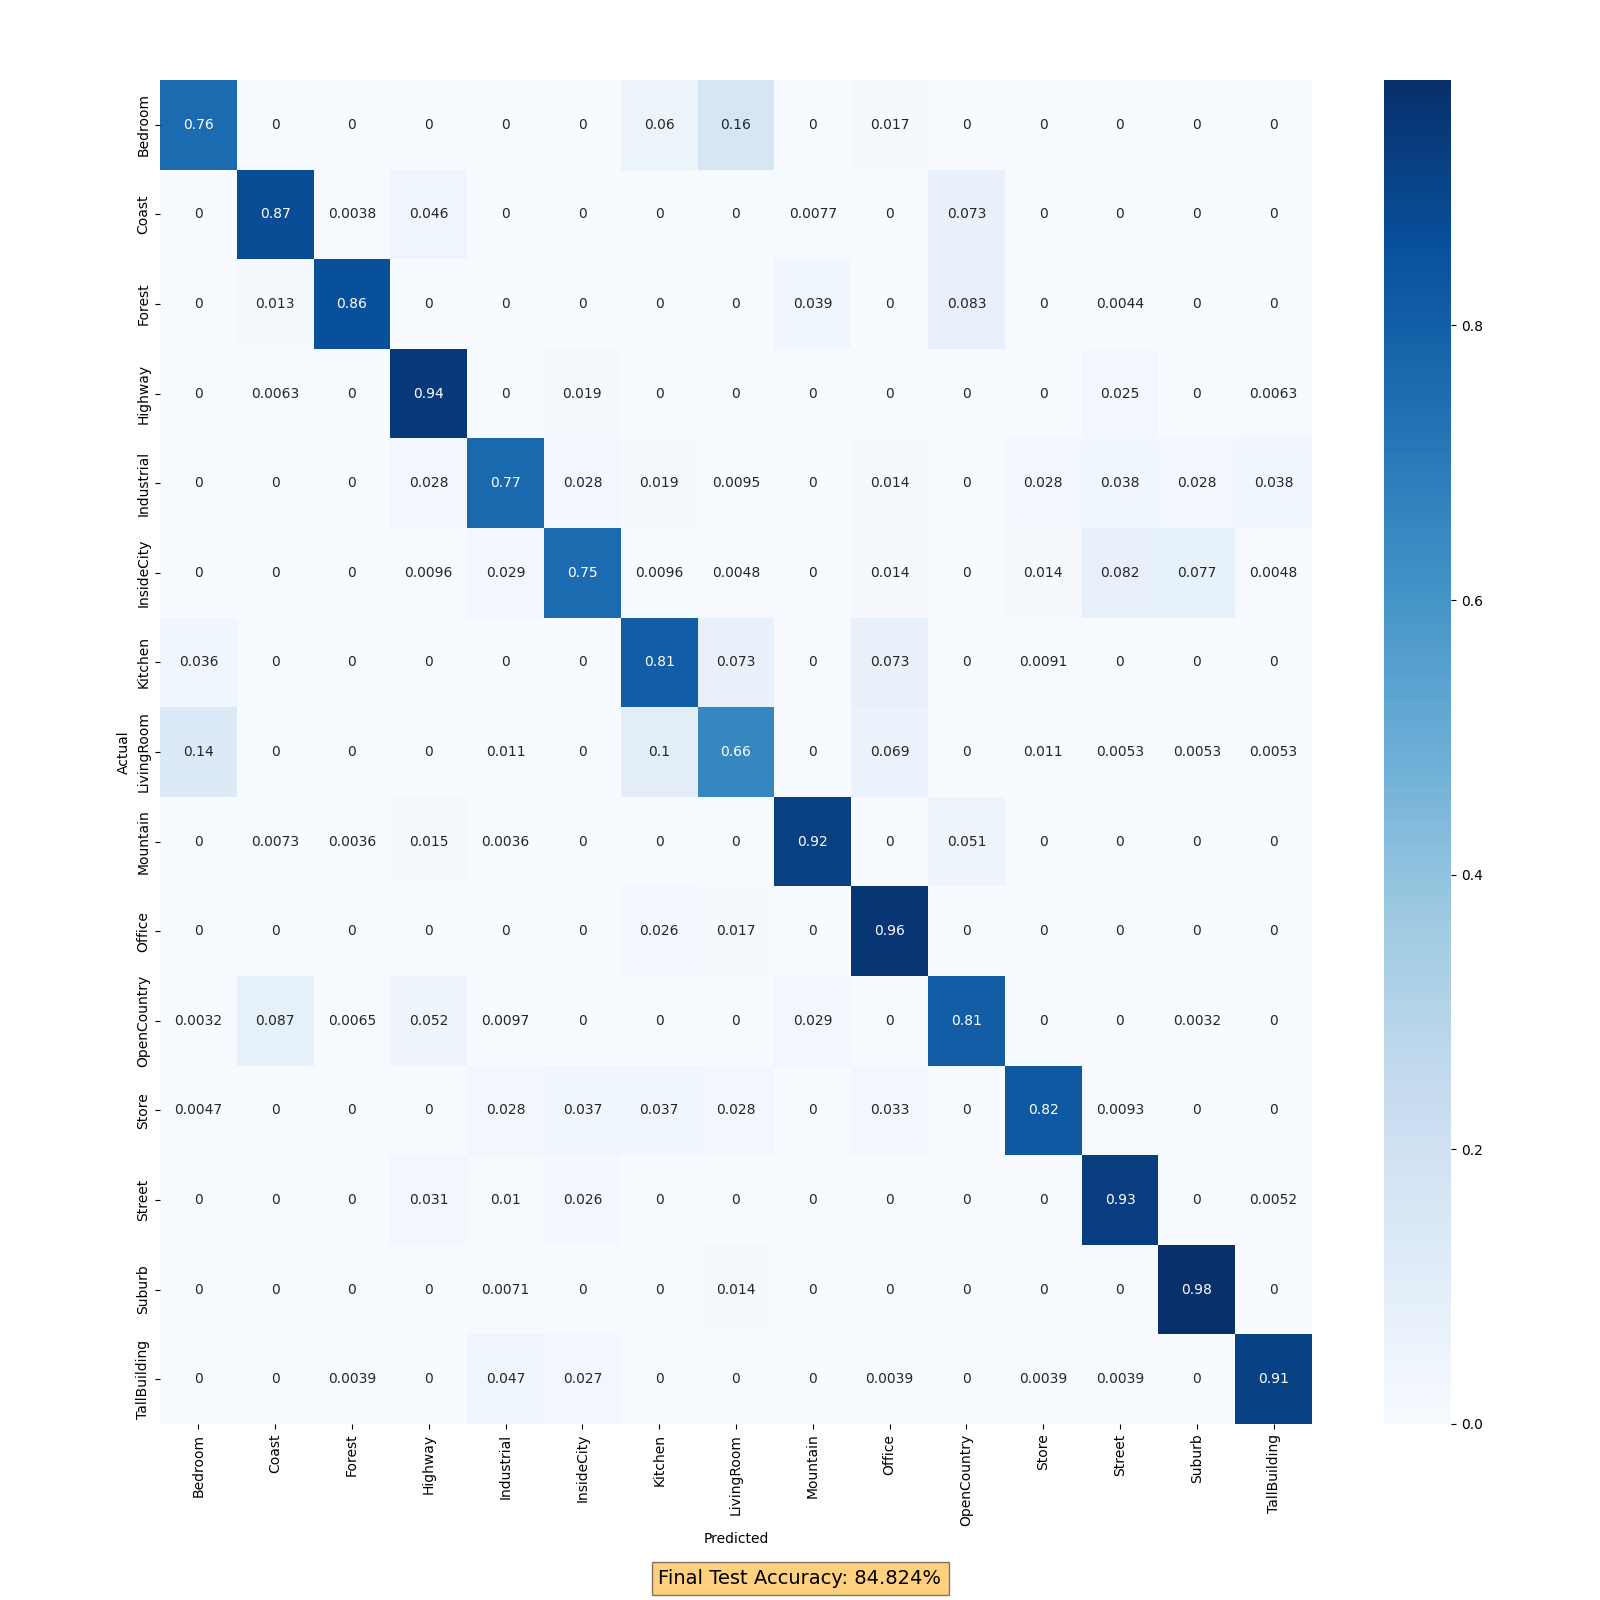
\includegraphics[width=.85\textwidth]{fig/confusion_matrix_task_3.png} \caption{Confusion matrix of the CNN classifier with AlexNet as a pretrained network on the test set.
}} 
  \end{figure}
  
It's a very good improvement from the previous tasks, in fact the test accuracy of the model is about 85\% and the model converges quickly.
From the confusion matrix it can be recognised that the model has a slight difficult classification problem with the two classes bedroom and living room and with coast and open country.





\newpage



\begin{thebibliography}{9}
\bibitem {Lazebnik:Crosa}
[Lazebnik et al., 2006] Lazebnik, S., Schmid, C., and Ponce, J. (2006). Beyond bags of features: Spatial pyramid matching for recognizing natural scene categories. In \emph{2006 IEEE computer society conference on computer vision and pattern recognition (CVPR'06),}, volume 2, pages 2169-2178.IEEE.

\bibitem {Ioffe:Szegedy}
[Ioffe and Szegedy, 2015] Ioffe, S. and Szegedy, C. (2015). Batch normalization:
Accelerating deep network training by reducing internal covariate shift. \emph{arXiv
preprint arXiv:1502.03167.}

\bibitem {Szegedy:Szegedy}
[Szegedy et al., 2015] Szegedy, C., Liu, W., Jia, Y., Sermanet, P., Reed, S.,
Anguelov, D., Erhan, D., Vanhoucke, V., and Rabinovich, A. (2015). Going
deeper with convolutions. In  \emph{The IEEE Conference on Computer Vision and
Pattern Recognition (CVPR).}

\bibitem {Krizhevsky:Krizhevsky}
[Krizhevsky et al., 2012] Krizhevsky, A., Sutskever, I., and Hinton, G. E.
(2012). Imagenet classification with deep convolutional neural networks. In \emph{Advances in neural information processing systems},pages 1097?1105.,



\end{thebibliography}

\end{document}
